Aside from insights into the security properties of \gls{prins} itself, modeling a complex protocol like this also provides a better understanding of the tool \textsc{ProVerif}.
The following is a brief account of some of the key challenges encountered while compiling this thesis.\medskip

Firstly, one of the most challenging aspects of the verification with \textsc{ProVerif} is the lack of built-in debug capabilities.
The reason why the debug queries in section~\ref{ssec:debug} are introduced to the verification is that without them, there is no indication when specified events cannot be reached individually.
Instead, compound reachability queries or correspondence assertions that incorporate these events are likely to provide erroneous results.
Without being aware of this behavior and explicitly testing the reachability of every single event itself, this may at times lead to a false confidence into the properties of the protocol.
Thankfully, the \textsc{ProVerif} user manual does mention using simple reachability queries to prevent exactly that (see \cite{blanchet2020proverif}, p.~52).
A lesson learned from facing the issue of certain protocol branches being unreachable is to add said debug queries from the very beginning of the modeling process each time a new event is specified.\medskip

Secondly, ensuring termination of the model checker is all but trivial and the tool provides little insights into situations that may lead to non-termination.
One commonly encountered issue during the verification of \gls{prins}, such as in the case of the query in listing~\ref{lst:query-sec-6}, is the program inserting an increasing number of rules during the resolution process when trying to prove a given fact is derivable from available clauses, but never succeeding to do so.
In other scenarios the program does not print out any indication of progress anymore and seemingly halts.

One source of this problem during verification was the confusion of sent and received messages between processes, leading to loops within the protocol.
As soon as the type signature of a \textsc{ProVerif} function matches those of the avilable names, the tool will attempt to execute it.
The recommended way to avoid such mix-ups is tagging the protocol using defined constants to guide the execution of honest protocol participants, as explained in the user manual by example of a cryptographic constructor (see \cite{blanchet2020proverif}, p.~114).
Key takeaway from the modeling experience of \gls{prins} is to add tags to every single input and any custom functions that may be ambiguous based on the type of their input arguments.

Beyond general best practices like the one above, \textsc{ProVerif} can offer little support to prevent non-termination, as termination analysis is generally an undecidable problem.
The configuration flag {\sffamily verboseTerm} which is supposed to enable a more detailed output with termination warnings does not yield any helpful results for the problematic queries.
Different built-in resolution strategies do not solve the problem either.\medskip

Thirdly, even if \textsc{ProVerif} itself successfully terminates and finds an attack, there is no guarantee the related trace can be exported in form of a visual graph.
By default, the program creates files of type \textit{dot} that can be consumed by the software Graphviz to draw a directed graph into several different output formats, such as pdf, png, or svg.
With large protocol models such as the one created for \gls{prins}, Graphviz's \textit{dot} utility is quickly overburdened by the number of nodes representing key protocol events and edges representing their relation as well as message flows.
As shown in figure~\ref{fig:dot-execution} after more than six hours of execution, Graphviz is still not able to completely render an attack trace from any of the disproven queries described in the previous sections.
Omitting all replications in the main process of the model, denoted by an exclamation mark, does not result in a noticable improvement.
Since \textit{dot} is the only utility in the Graphviz toolbox that produces directed graphs, the output of other programs such as \textit{sfdp} or \textit{neato} which do terminate is not suitable to retrace the protocol execution either.
A question on how these issues may be resolved posted to the official \textsc{ProVerif} mailing list did not result in further insights until the date of submission.
Hence, the only result provided for queries 8, 9, and 10 is the textual representation of the attack trace by \textsc{ProVerif} and the raw dot files.

\begin{figure}[h!]
    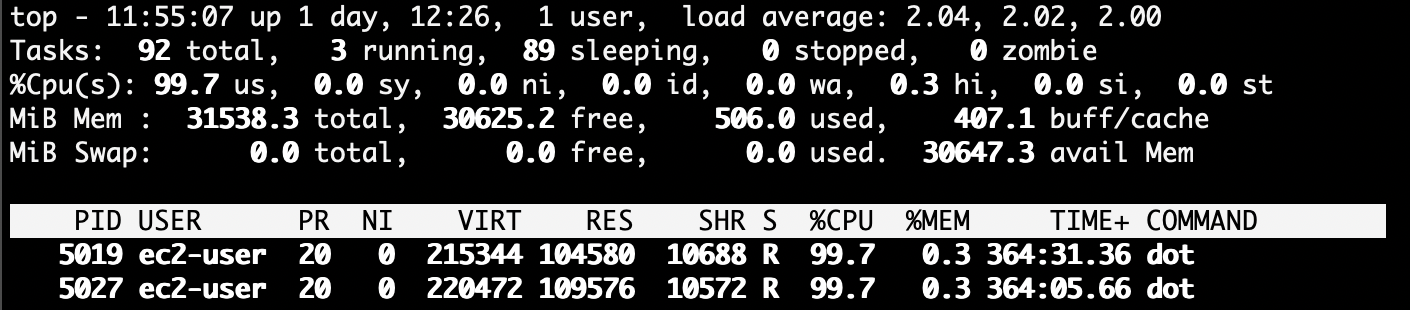
\includegraphics[width=\textwidth]{dot-execution.png}
    \centering
    \caption{Graphviz dot utility execution}
    \label{fig:dot-execution}
\end{figure}

Since \textit{dot} is the only supported output for a visual representation of the discovered attack traces, \textsc{ProVerif} is necessarily limited by the issues with the handling of this file format.
The lack of such visualization severely complicates validation of the discovered attacks.
It should be noted that \textsc{ProVerif} still prints a text-based description of the attack trace on the standard output.
However, given the large amounts of system states this representation is quickly becoming unmanagable for complex protocols itself.\medskip

Fourthly, unlike in many popular programming languages, the behavior of constructurs and destructors within an if-then-else clause is such that they do not produce a boolean negative return value in case of failure, but the special value {\sffamily fail}.
This can easily lead to unintended behavior as neither of the branches of the logic tree are executed and instead the process as a whole fails.
What is more, \textsc{ProVerif's} output does not contain any warnings about failed constructors, destructors, and processes.
Listing \ref{lst:patch-verification} shows a possible way to prevent this behavior by example of the destructor used to verify signed \gls{json} patches by \gls{ipx} providers.
The definition is structured two parts: the function signature, indicating the input and output types as well as a sequence of several different rewrite rules.
The first one indicates the positive case, including a well-formed \gls{json} patch object that has been signed with the same private key as the one belonging to the public key the signature is verified with.
In this case, the return value is true.
If the definition of the deconstructor would finish at this point, the different possible failures would not be catered for.
Hence, the next line starting with the keyword {\sffamily otherwise} captures scenarios in which the private/public key pair is not matching.
The last {\sffamily otherwise} branch is a catch-all rule, capturing cases in which the first input parameter does not match the expected structure of a \gls{json} patch.

\begin{lstlisting}[caption={Custom channel declarations},label={lst:patch-verification},firstnumber=23]
fun validPrinsSign(bitstring, pubkey): bool
reduc forall p: prins, ops: bitstring, id: bitstring, tag: mac, k: privkey;
    validPrinsSign(signPrins(p, ops, id, tag, k), pk(k)) = true
otherwise forall p: prins, ops: bitstring, id: bitstring, tag: mac,
    k: privkey, k': privkey;
    validPrinsSign(signPrins(p, ops, id, tag, k'), pk(k)) = false
otherwise forall k: privkey;
    validPrinsSign(fail, pk(k)) = false.
\end{lstlisting}


Lastly, \textsc{ProVerif}'s lack of support for multi-threaded execution can become a bottleneck when verifying larger systems.
Given that the software only ever makes use of a single thread at once, each query is executed sequentially and a blocking query will block all remain ones indefinitely.
This is especially problematic when the protocol under test has reached a sizable complexity and existing queries are modified or new queries are added in later stages.

In these situations, splitting up the set of queries into different \textsc{ProVerif} files lends itself as a crude method of macro-parallelization.
While effective, this practice is tedious and time-consuming.
Ideally, \textsc{ProVerif} would add a command line option that would allow to distribute queries across several threads.
Likewise, a simple optimization related to the generation of attack traces explained above, would be spawning the \textit{dot} process in parallel to \textsc{ProVerif} itself.
That way, in contrast to the current implementation, the time-consuming rendering of these graphs would not block the verification as a whole.\medskip

All in all, the above issues related to the reporting of warnings and internal progress during verification, program non-termination, and the visualization of discovered attack traces render the obtained results vague at best.
Without a practical way to retrace the executed procotol flow, verifying \textsc{ProVerif}'s findings, let alone deriving improvements for the protocol based on them, is simply unfeasible.
The program's interactive mode is aimed at addressing this requirement, but handicaped by limited feature support as well, since it only allows structuring protocols using phases, not synchronozation groups as employed by the created model.
However, it has to be acknowledged that the underlying problem, that is verifying the models correctness in terms of accurately representing the specification, is something that the tool itself cannot provide unless the specification is not written in a formal way in the first place.
This is not the case with the 5G security specification \gls{ts} 33.501 or any other \gls{3gpp} document.